\documentclass[10pt, letterpaper]{article}
% Packages:
\usepackage[
    ignoreheadfoot, % set margins without considering header and footer
    top=2 cm, % seperation between body and page edge from the top
    bottom=2 cm, % seperation between body and page edge from the bottom
    left=2 cm, % seperation between body and page edge from the left
    right=2 cm, % seperation between body and page edge from the right
    footskip=1.0 cm, % seperation between body and footer
    % showframe % for debugging 
]{geometry} % for adjusting page geometry
\usepackage{titlesec} % for customizing section titles
\usepackage{tabularx} % for making tables with fixed width columns
\usepackage{array} % tabularx requires this
\usepackage[dvipsnames]{xcolor} % for coloring text
\definecolor{primaryColor}{RGB}{0, 79, 144} % define primary color
\usepackage{enumitem} % for customizing lists
\usepackage{fontawesome5} % for using icons
\usepackage{amsmath} % for math
\usepackage[
    pdftitle={Matteo Romilio Pasqual's CV},
    pdfauthor={Matteo Romilio Pasqual},
    pdfcreator={LaTeX with RenderCV},
    colorlinks=true,
    urlcolor=primaryColor
]{hyperref} % for links, metadata and bookmarks
\usepackage[pscoord]{eso-pic} % for floating text on the page
\usepackage{calc} % for calculating lengths
\usepackage{bookmark} % for bookmarks
\usepackage{lastpage} % for getting the total number of pages
\usepackage{changepage} % for one column entries (adjustwidth environment)
\usepackage{paracol} % for two and three column entries
\usepackage{ifthen} % for conditional statements
\usepackage{needspace} % for avoiding page brake right after the section title
\usepackage{iftex} % check if engine is pdflatex, xetex or luatex
\usepackage{etoolbox}
\usepackage{graphicx} % for including the profile photo
\usepackage{tikz} % for the circular photo crop

% Ensure that generate pdf is machine readable/ATS parsable:
\ifPDFTeX
    \input{glyphtounicode}
    \pdfgentounicode=1
    % \usepackage[T1]{fontenc} % this breaks sb2nov
    \usepackage[utf8]{inputenc}
    \usepackage{lmodern}
\fi
% Some settings:
\AtBeginEnvironment{adjustwidth}{\partopsep0pt} % remove space before adjustwidth environment
\pagestyle{empty} % no header or footer
\setcounter{secnumdepth}{0} % no section numbering
\setlength{\parindent}{0pt} % no indentation
\setlength{\topskip}{0pt} % no top skip
\setlength{\columnsep}{0cm} % set column seperation
\makeatletter
\let\ps@customFooterStyle\ps@plain % Copy the plain style to customFooterStyle
\patchcmd{\ps@customFooterStyle}{\thepage}{
    \color{gray}\textit{\small Matteo Romilio Pasqual - Page \thepage{} of \pageref*{LastPage}}
}{}{} % replace number by desired string
\makeatother
\pagestyle{customFooterStyle}
\titleformat{\section}{\needspace{4\baselineskip}\bfseries\large}{}{0pt}{}[\vspace{1pt}\titlerule]
\titlespacing{\section}{-1pt}{0.3 cm}{0.2 cm} % section title spacing
\renewcommand\labelitemi{$\circ$} % custom bullet points
\newenvironment{highlights}{
    \begin{itemize}[
        topsep=0.10 cm,
        parsep=0.10 cm,
        partopsep=0pt,
        itemsep=0pt,
        leftmargin=0.4 cm + 10pt
    ]
}{
    \end{itemize}
} % new environment for highlights
\newenvironment{highlightsforbulletentries}{
    \begin{itemize}[
        topsep=0.10 cm,
        parsep=0.10 cm,
        partopsep=0pt,
        itemsep=0pt,
        leftmargin=10pt
    ]
}{
    \end{itemize}
} % new environment for highlights for bullet entries
\newenvironment{onecolentry}{
    \begin{adjustwidth}{
        0.2 cm + 0.00001 cm
    }{
        0.2 cm + 0.00001 cm
    }
}{
    \end{adjustwidth}
} % new environment for one column entries
\newenvironment{twocolentry}[2][]{
    \onecolentry
    \def\secondColumn{#2}
    \setcolumnwidth{\fill, 4.5 cm}
    \begin{paracol}{2}
}{
    \switchcolumn \raggedleft \secondColumn
    \end{paracol}
    \endonecolentry
} % new environment for two column entries
\newenvironment{header}{
    \setlength{\topsep}{0pt}\par\kern\topsep\centering\linespread{1.5}
}{
    \par\kern\topsep
} % new environment for the header
\newcommand{\placelastupdatedtext}{% \placetextbox{<horizontal pos>}{<vertical pos>}{<stuff>}
  \AddToShipoutPictureFG*{% Add <stuff> to current page foreground
    \put(
        \LenToUnit{\paperwidth-2 cm-0.2 cm+0.05cm},
        \LenToUnit{\paperheight-1.0 cm}
    ){\vtop{{\null}\makebox[0pt][c]{
        \small\color{gray}\textit{Last updated in September 2024}\hspace{\widthof{Last updated in September 2024}}
    }}}%
  }%
}%
% NOTE: replace "photo.jpg" below with your actual photo filename
% (keep the file in the same folder as this .tex file, or give a full path).
% The photo width can be adjusted here:
\newcommand{\profilephotowidth}{3.5 cm}
% save the original href command in a new command:
\let\hrefWithoutArrow\href
% new command for external links:
\renewcommand{\href}[2]{\hrefWithoutArrow{#1}{\ifthenelse{\equal{#2}{}}{ }{#2 }\raisebox{.15ex}{\footnotesize \faExternalLink*}}}
\begin{document}
\newcommand{\AND}{\unskip\cleaders\copy\ANDbox\hskip\wd\ANDbox\ignorespaces}
\newsavebox\ANDbox
\sbox\ANDbox{}

%--------------------------HEADER----------------------------------------------
\noindent
\begin{minipage}[c]{\profilephotowidth}
    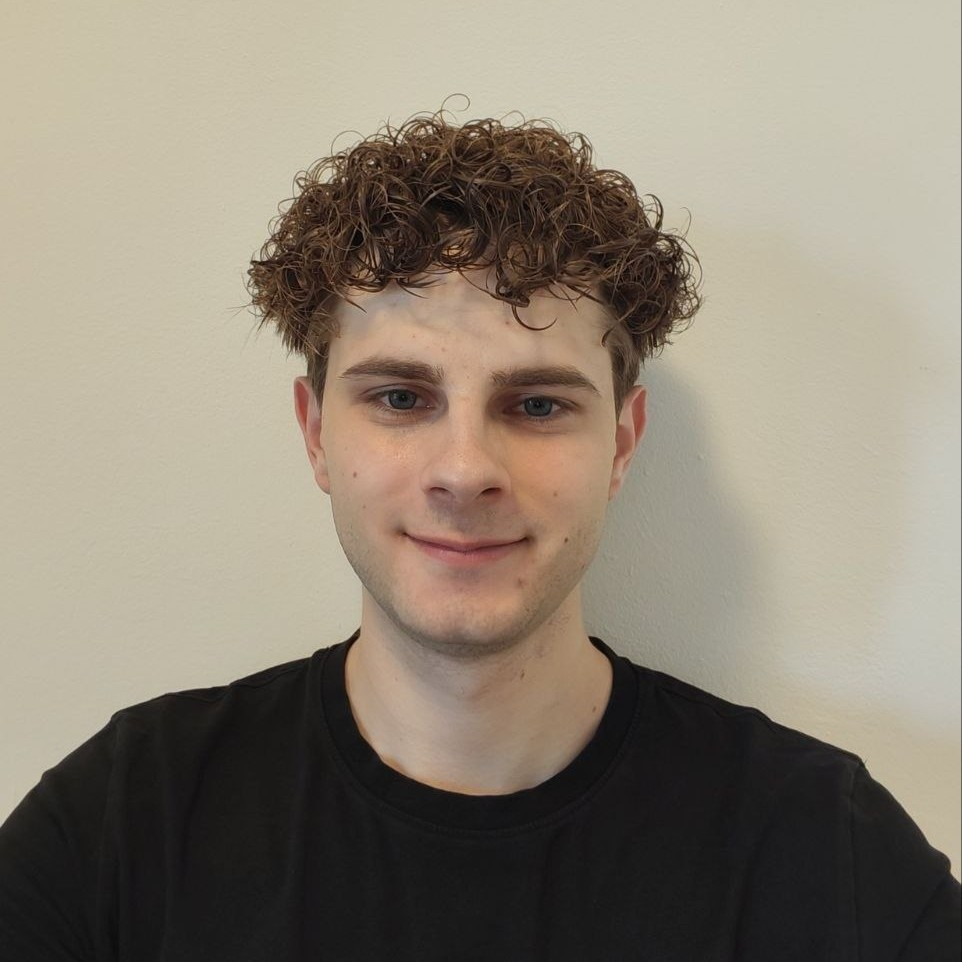
\includegraphics[width=\profilephotowidth]{photo.jpg}
\end{minipage}%
\hfill
\begin{minipage}[c]{\dimexpr\textwidth-\profilephotowidth-0.4cm\relax}
\begin{header}
    \textbf{\fontsize{24 pt}{24 pt}\selectfont Matteo Romilio Pasqual}
        
    \vspace{0.3 cm}
        
    \normalsize
    \mbox{{\color{black}\footnotesize\faMapMarker*}\hspace*{0.13cm}Milan (IT)}%
    \kern 0.25 cm%
    \AND%
    \kern 0.25 cm
    \mbox{\hrefWithoutArrow{mailto:matteoromilio.pasqual@mail.polimi.it}{\color{black}{\footnotesize\faEnvelope[regular]}\hspace*{0.13cm}matteoromilio.pasqual@mail.polimi.it}}%
    \kern 0.25 cm
    \AND \\ \vspace{-0.3 cm}
    \kern 0.25 cm
    \mbox{\hrefWithoutArrow{https://www.linkedin.com/in/matteo-romilio-pasqual/}{\color{black}{\footnotesize\faLinkedinIn}\hspace*{0.13cm}Matteo Pasqual}}%
    \kern 0.25 cm
    \AND
    \kern 0.25 cm
    \mbox{\hrefWithoutArrow{https://github.com/matteopasqual02}{\color{black}{\footnotesize\faGithub}\hspace*{0.13cm}matteopasqual02}}

    "In the middle of difficulty lies opportunity." – Albert Einstein
        
\end{header}
\end{minipage}
\vspace{0.3 cm - 0.3 cm}

%--------------------------EDUCATION----------------------------------------------
\section{\mbox{{\color{black}\footnotesize\faGraduationCap}\hspace*{0.13cm}Education}}
    
    \begin{twocolentry}{    
    \textit{Sep 2024 – Jul 2026}}
    \textbf{Politecnico di Milano (\href{https://www.polimi.it/}{polimi.it})}
    \end{twocolentry}
    \begin{onecolentry}
    M.Sc. in Computer Science and Engineering - Artificial intelligence \hspace{20pt}Grade: 110L/110
    \end{onecolentry}   

    \vspace{0.10 cm}
    \begin{twocolentry}{
    \textit{Sep 2021 – Jul 2024}}
    \textbf{Politecnico di Milano (\href{https://www.polimi.it/}{polimi.it})}
    \end{twocolentry}
    \begin{onecolentry}
    B.Sc. in Computer Science and Engineering \hspace{1pt} \hspace{119pt}Grade: 109/110
    \end{onecolentry}

    \vspace{0.10 cm}
    \begin{twocolentry}{
    \textit{Sep 2016 – Jul 2021}}
    \textbf{Liceo Scientifico "Leonardo da Vinci" (\href{https://www.liceogallarate.edu.it/} {liceogallarate.it})}
    \end{twocolentry}
    \begin{onecolentry}
    Diploma di Liceo Scientifico - Scienze Applicate \hspace{1pt} \hspace{102pt}Grade: 96/100
    \end{onecolentry}



%--------------------------RESEARCH----------------------------------------------
\section{\mbox{{\color{black}\footnotesize\faReact}\hspace*{0.13cm}Projects and Research}}

\vspace{0.10 cm}
\begin{twocolentry}{\textit{Master Thesis - 2026}}
\textbf{M-SHRED: Masked Shallow Recurrent Decoders \\ for Fault-Tolerant Sparse Sensing under Missing Sensor Measurements}
\end{twocolentry}

\vspace{0.10 cm}
\begin{onecolentry}
\begin{highlights}
    \item Designed and validated a hierarchy of Transformer-based masking mechanisms to make sparse-sensing reconstruction models explicitly aware of missing sensor data, and introduced a multi-step decoding training strategy that further improved reconstruction accuracy and latent trajectory smoothness, with no additional inference-time overhead
    \item Gained hands-on research experience in deep learning and reduced-order modeling, alongside strengthened skills in experimental design, scientific writing, and end-to-end reproducible ML research on both synthetic and real-world noisy datasets
\end{highlights}
\end{onecolentry}

\vspace{0.20 cm}
\begin{twocolentry}{\textit{Challenge - 2025}}
    \textbf{Multi-agent System Leonardo Drone Contest 2025}
\end{twocolentry}
\vspace{0.10 cm}
\begin{onecolentry}
    \begin{highlights}         
        \item Ranked 2nd nationally in a robotics competition (\href{https://www.leonardo.com/it/innovation-technology/open-innovation/drone-contest}{LDC-2025}) among teams from top Italian universities
        \item Developed planning, exploration, and localization algorithms for a collaborative rover-drone system, together with computer vision modules for ArUco/QR marker detection and unknown object detection, to dynamically execute and reschedule mission tasks in real time based on external triggers
        \item Achieved reliable autonomous target and object detection, marker-sequence following, and coordinated rover-drone task hand-off, validating the robustness of the proposed planning and perception pipeline under dynamic, real-time mission constraints
    \end{highlights}
\end{onecolentry}

\vspace{0.20 cm}
\begin{twocolentry}{\textit{Projects - 2025}}
    \textbf{Course Projects}
\end{twocolentry}

\vspace{0.10 cm}
\begin{onecolentry}
    \begin{highlights}
        \item Artificial Neural Networks and Deep Learning (ANNDL) course project: multivariate time-series classification using neural networks (\href{https://github.com/Gradient-Gang/ANN-Challenges.git}{GitHub})
        \item Artificial Neural Networks and Deep Learning (ANNDL) course project: biomedical image classification using deep learning methods (\href{https://github.com/Gradient-Gang/ANN-Challenge-2.git}{GitHub})
        \item Mathematical Models and Methods for Image Processing (MMMIP) course project: image processing for denoising, inpainting, and anomaly detection (\href{https://github.com/matteopasqual02/MMMIP-2025-homeworks.git}{GitHub})
        \item Online Learning Applications (OLA) course project: pricing under budget constraints using online learning methods (\href{https://github.com/matteopasqual02/OLA-2025-project.git}{GitHub})
    \end{highlights}
\end{onecolentry}

\vspace{0.20 cm}
\begin{twocolentry}{\textit{Project - 2024}}
    \textbf{Kolmogorov-Arnold Networks (KANs) lecture}
\end{twocolentry}
\vspace{0.10 cm}
\begin{onecolentry}
    \begin{highlights}
        \item Studied and presented Kolmogorov-Arnold Networks (KANs), a spline-based alternative to MLPs inspired by the Kolmogorov-Arnold theorem, as part of the Numerical Analysis for Machine Learning course
        \item Analyzed KANs' theoretical foundations and architectural differences from MLPs, covering learnable B-spline activation functions, training dynamics, and advanced techniques (sparsification, pruning, symbolic regression) for improved interpretability
        \item Implemented and benchmarked KANs on regression and real-world classification tasks, achieving a higher classification accuracy, and published the code and materials (\href{https://github.com/matteopasqual02/KAN-naml.git}{GitHub})
    \end{highlights}
\end{onecolentry}

\vspace{0.20 cm}
\begin{twocolentry}{\textit{Research - 2024}}
    \textbf{Non-intrusive Monitoring of Daily Habits in Older Adults: \\ A Chaos Game Representation-Based Approach}
\end{twocolentry}
\vspace{0.10 cm}
\begin{onecolentry}
    \begin{highlights}
        \item Published a short paper at UCAmI 2025 -- 17th International Conference on Ubiquitous Computing and Ambient Intelligence (\href{https://doi.org/10.1007/978-3-032-16992-1_20}{DOI})
        \item Developed a novel framework using Chaos Game Representation (CGR) to transform time-series sensor data into fractal-like images for behavioural analysis, enabling classification of daily routines
        \item Demonstrated effective anomaly detection and clustering of behavioural patterns on both synthetic and real-world multi-resident datasets
    \end{highlights}
\end{onecolentry}

%--------------------------PUBLICATIONS----------------------------------------------

\section{\mbox{{\color{black}\footnotesize\faBook}\hspace*{0.13cm}Publications}}

\begin{onecolentry}
\textbf{Non-intrusive Monitoring of Daily Habits in Older Adults: \\ A Chaos Game Representation-Based Approach}

UCAmI 2025 -- 17th International Conference on Ubiquitous Computing and Ambient Intelligence (\href{https://doi.org/10.1007/978-3-032-16992-1_20}{DOI})
\end{onecolentry}

%--------------------------EXPERIENCE----------------------------------------------
\section{\mbox{{\color{black}\footnotesize\faShoePrints}\hspace*{0.13cm}Experience}}

    \begin{twocolentry}{
    \textit{Milano, IT}    
            
    \textit{Sep 2025 – Jul 2026}}
    \textbf{University Multichance Tutor}
            
    \textit{Politecnico di Milano}
    \end{twocolentry}
    \vspace{0.10 cm}
    \begin{onecolentry}
    \begin{highlights}
        \item Provided one-to-one academic tutoring to university students through the Multichance program
        \item Provided personalized academic support and study assistance
    \end{highlights}
    \end{onecolentry}

\vspace{0.20 cm}

    \begin{twocolentry}{
    \textit{Milano, IT}    
            
    \textit{Sep 2022 – Jul 2024}}
    \textbf{University Peer-to-peer Tutor}
            
    \textit{Politecnico di Milano}
    \end{twocolentry}
    \vspace{0.10 cm}
    \begin{onecolentry}
    \begin{highlights}
        \item Provided one-to-one academic tutoring to university students through the Peer-to-Peer tutoring program
        \item Provided personalized academic support and study assistance
    \end{highlights}
    \end{onecolentry}

%--------------------------LANGUAGES----------------------------------------------    
\section{\mbox{{\color{black}\footnotesize\faGlobeAmericas}\hspace*{0.13cm}Languages}}

\begin{highlights}
    \item \textbf{Italian}: Native
    \item \textbf{English}: Upper Intermediate (B2+)
\end{highlights}

%--------------------------SKILLS----------------------------------------------
\section{\mbox{{\color{black}\footnotesize\faWrench}\hspace*{0.13cm}Skills}}

    \begin{samepage}
    \begin{highlights}
        \item \textbf{AI \& Machine Learning}: PyTorch, TensorFlow/Keras, scikit-learn, OpenCV
        \item \textbf{Programming \& Software Dev.}: Python, C/C++, Java
        \item \textbf{Databases Technologies}: SQL, MongoDB, Spark, Neo4j, Zilliz-Milvus, Pandas
        \item \textbf{OS \& Middleware}: ROS, ROS2, Linux, Docker and VMs
        \item \textbf{Other Technologies}: Matlab, VHDL/Vivado,  Git/GitHub, \LaTeX
    \end{highlights}
    \end{samepage}

%--------------------------AWARDS----------------------------------------------  
\section{\mbox{{\color{black}\footnotesize\faTrophy}\hspace*{0.13cm}Awards}}
        \begin{twocolentry}{2023}
            \textbf{Best Freshmen Award}: top 5\% freshmen of PoliMi
        \end{twocolentry}

%--------------------------Volunteering---------------------------------------------- 
    \section{\mbox{{\color{black}\footnotesize\faSeedling}\hspace*{0.13cm}Volunteering}}
            
        \begin{twocolentry}{Sep 2016 - Aug 2021}
        \textbf{Volunteer at Oratorio di Albizzate}\\
        Albizzate
        \end{twocolentry}
        \begin{highlights}
    \item Organized educational, recreational, and community activities for children and teenagers
\end{highlights}

\end{document}